\documentclass{beamer}  
\usepackage[T1]{fontenc}
\usepackage{xcolor}
\usepackage{mathtools}
\usepackage{graphicx}
\usepackage{subcaption}
\usepackage[edges]{forest}
\usepackage{listings}
\usepackage{xcolor}

\definecolor{codegreen}{rgb}{0,0.6,0}
\definecolor{codegray}{rgb}{0.5,0.5,0.5}
\definecolor{codepurple}{rgb}{0.58,0,0.82}
\definecolor{backcolour}{rgb}{1, 1, 1}

\lstdefinestyle{pythonstyle}{
	backgroundcolor=\color{backcolour},
	commentstyle=\color{codegreen},
	keywordstyle=\color{blue}\bfseries,
	numberstyle=\tiny\color{codegray},
	stringstyle=\color{codepurple},
	basicstyle=\ttfamily\footnotesize,
	breakatwhitespace=false,
	breaklines=true,
	captionpos=b,
	keepspaces=true,
	numbers=left,
	showspaces=false,
	showstringspaces=false,
	showtabs=false,
	tabsize=2,
	language=Python
}

\usefonttheme[onlymath]{serif}
\renewcommand\sfdefault{cmtt}

\usecolortheme[named=black]{structure}
\setbeamercolor{normal text}{fg=black}
\setbeamercolor{structure}{fg=black}
\setbeamercolor{section in toc}{fg=black}

\title{intro to mathematics in software engineering}
\institute{Fontys University of Applied Sciences}
\date{\today}

\begin{document}
	
	% title-page
	\begin{frame}
		\titlepage
	\end{frame}
	
	% objectives
	\begin{frame}{objectives}
		\begin{itemize}
			\item[] scary looking functions
			\item[] math related software engineering concepts
			\item[] translate math to programming
		\end{itemize}
	\end{frame}
	
	% fundamentals-1
	\begin{frame}{fundamentals of mathematical and function notation}
		$$f(x)=x^2$$
	\end{frame}
	
	% fundamentals-2
	\begin{frame}{fundamentals of mathematical and function notation}
		\begin{itemize}
			\item[] $a\cdot f(x)$
			\item[]
			\item[] $f(x/b)$
			\item[]
			\item[] $f(x-c)$
			\item[]
			\item[] $f(x)+d$
		\end{itemize}
	\end{frame}
	
	% fundamentals-3
	\begin{frame}{fundamentals of mathematical and function notation}
		\begin{itemize}
			\item[] $a\cdot f(x) \Rightarrow \text{multiplies the y-value by } a$
			\item[]
			\item[] $f(x/b) \Rightarrow \text{multiplies the x-value by } b$
			\item[]
			\item[] $f(x-c) \Rightarrow \text{shifts graph } c \text{ units to the right}$
			\item[]
			\item[] $f(x)+d \Rightarrow \text{shifts graph } d \text{ units upward}$
		\end{itemize}
	\end{frame}

	% breakdown-1
	\begin{frame}{breaking down a scary looking function}
		\vfill
		\begin{center}
			$$g(x)=\frac{4}{\pi}\sum_{n=1}^{\infty}\frac{\sin(2\pi (2n-1)ft)}{2n-1}$$
		\end{center}
		\vfill
		\begin{center}
			\small (where $t = \text{time},\ f = \text{frequency},\ n = \text{iterations}$)
		\end{center}
		\vfill
	\end{frame}

	
	% breakdown-2
	\begin{frame}{breaking down a scary looking function}
		\vfill
		\begin{center}
			$$g(x) = \frac{4}{\pi}\colorbox{red!20}{$\displaystyle \sum_{n=1}^{\infty}$}\frac{\sin(2\pi(2n-1)ft)}{2n-1}$$
		\end{center}
		\vfill
		\begin{center}
			we are dealing with a function built from multiple smaller functions added together
		\end{center}
		\vfill
	\end{frame}

	
	% breakdown-3
	\begin{frame}{breaking down a scary looking function}
		\vfill
		\begin{center}
			$$g(x)=\frac{4}{\pi}\sum_{n=1}^{\infty}\frac{\colorbox{red!20}{$\displaystyle \sin$}(2\pi (2n-1)ft)}{2n-1}$$
		\end{center}
		\vfill
		\begin{center}
			the $sin$ on the inside suggests we are dealing with waves or oscillations
		\end{center}
		\vfill
	\end{frame}
	
	% breakdown-4
	\begin{frame}{breaking down a scary looking function}
		\vfill
		\begin{center}
			$$g(x)=\frac{4}{\pi}\sum_{n=1}^{\infty}\frac{\sin(2\pi (2n-1)ft)}{\colorbox{red!20}{$\displaystyle 2n-1$}}$$
		\end{center}
		\vfill
		\begin{center}
			denominator \(2n-1\) hints that terms get smaller as \(n\) increases — later terms have less influence
		\end{center}
		\vfill
	\end{frame}

	
	% breakdown-5
	\begin{frame}{breaking down a scary looking function}
		$$g_{1}(t)=\frac{4}{\pi}\cdot \frac{\sin(2\pi (2(1)-1)ft)}{2(1)-1}$$
		$$=\frac{4}{\pi}\cdot \frac{\sin(2\pi (1)ft)}{1}$$
		$$=\frac{4}{\pi}\cdot\sin(2\pi ft)$$
		$$g_{1}(t)=\colorbox{green!20}{$\displaystyle \frac{4}{\pi}\sin(2\pi ft)$}$$
	\end{frame}
	
	% breakdown-6
	\begin{frame}{breaking down a scary looking function}
		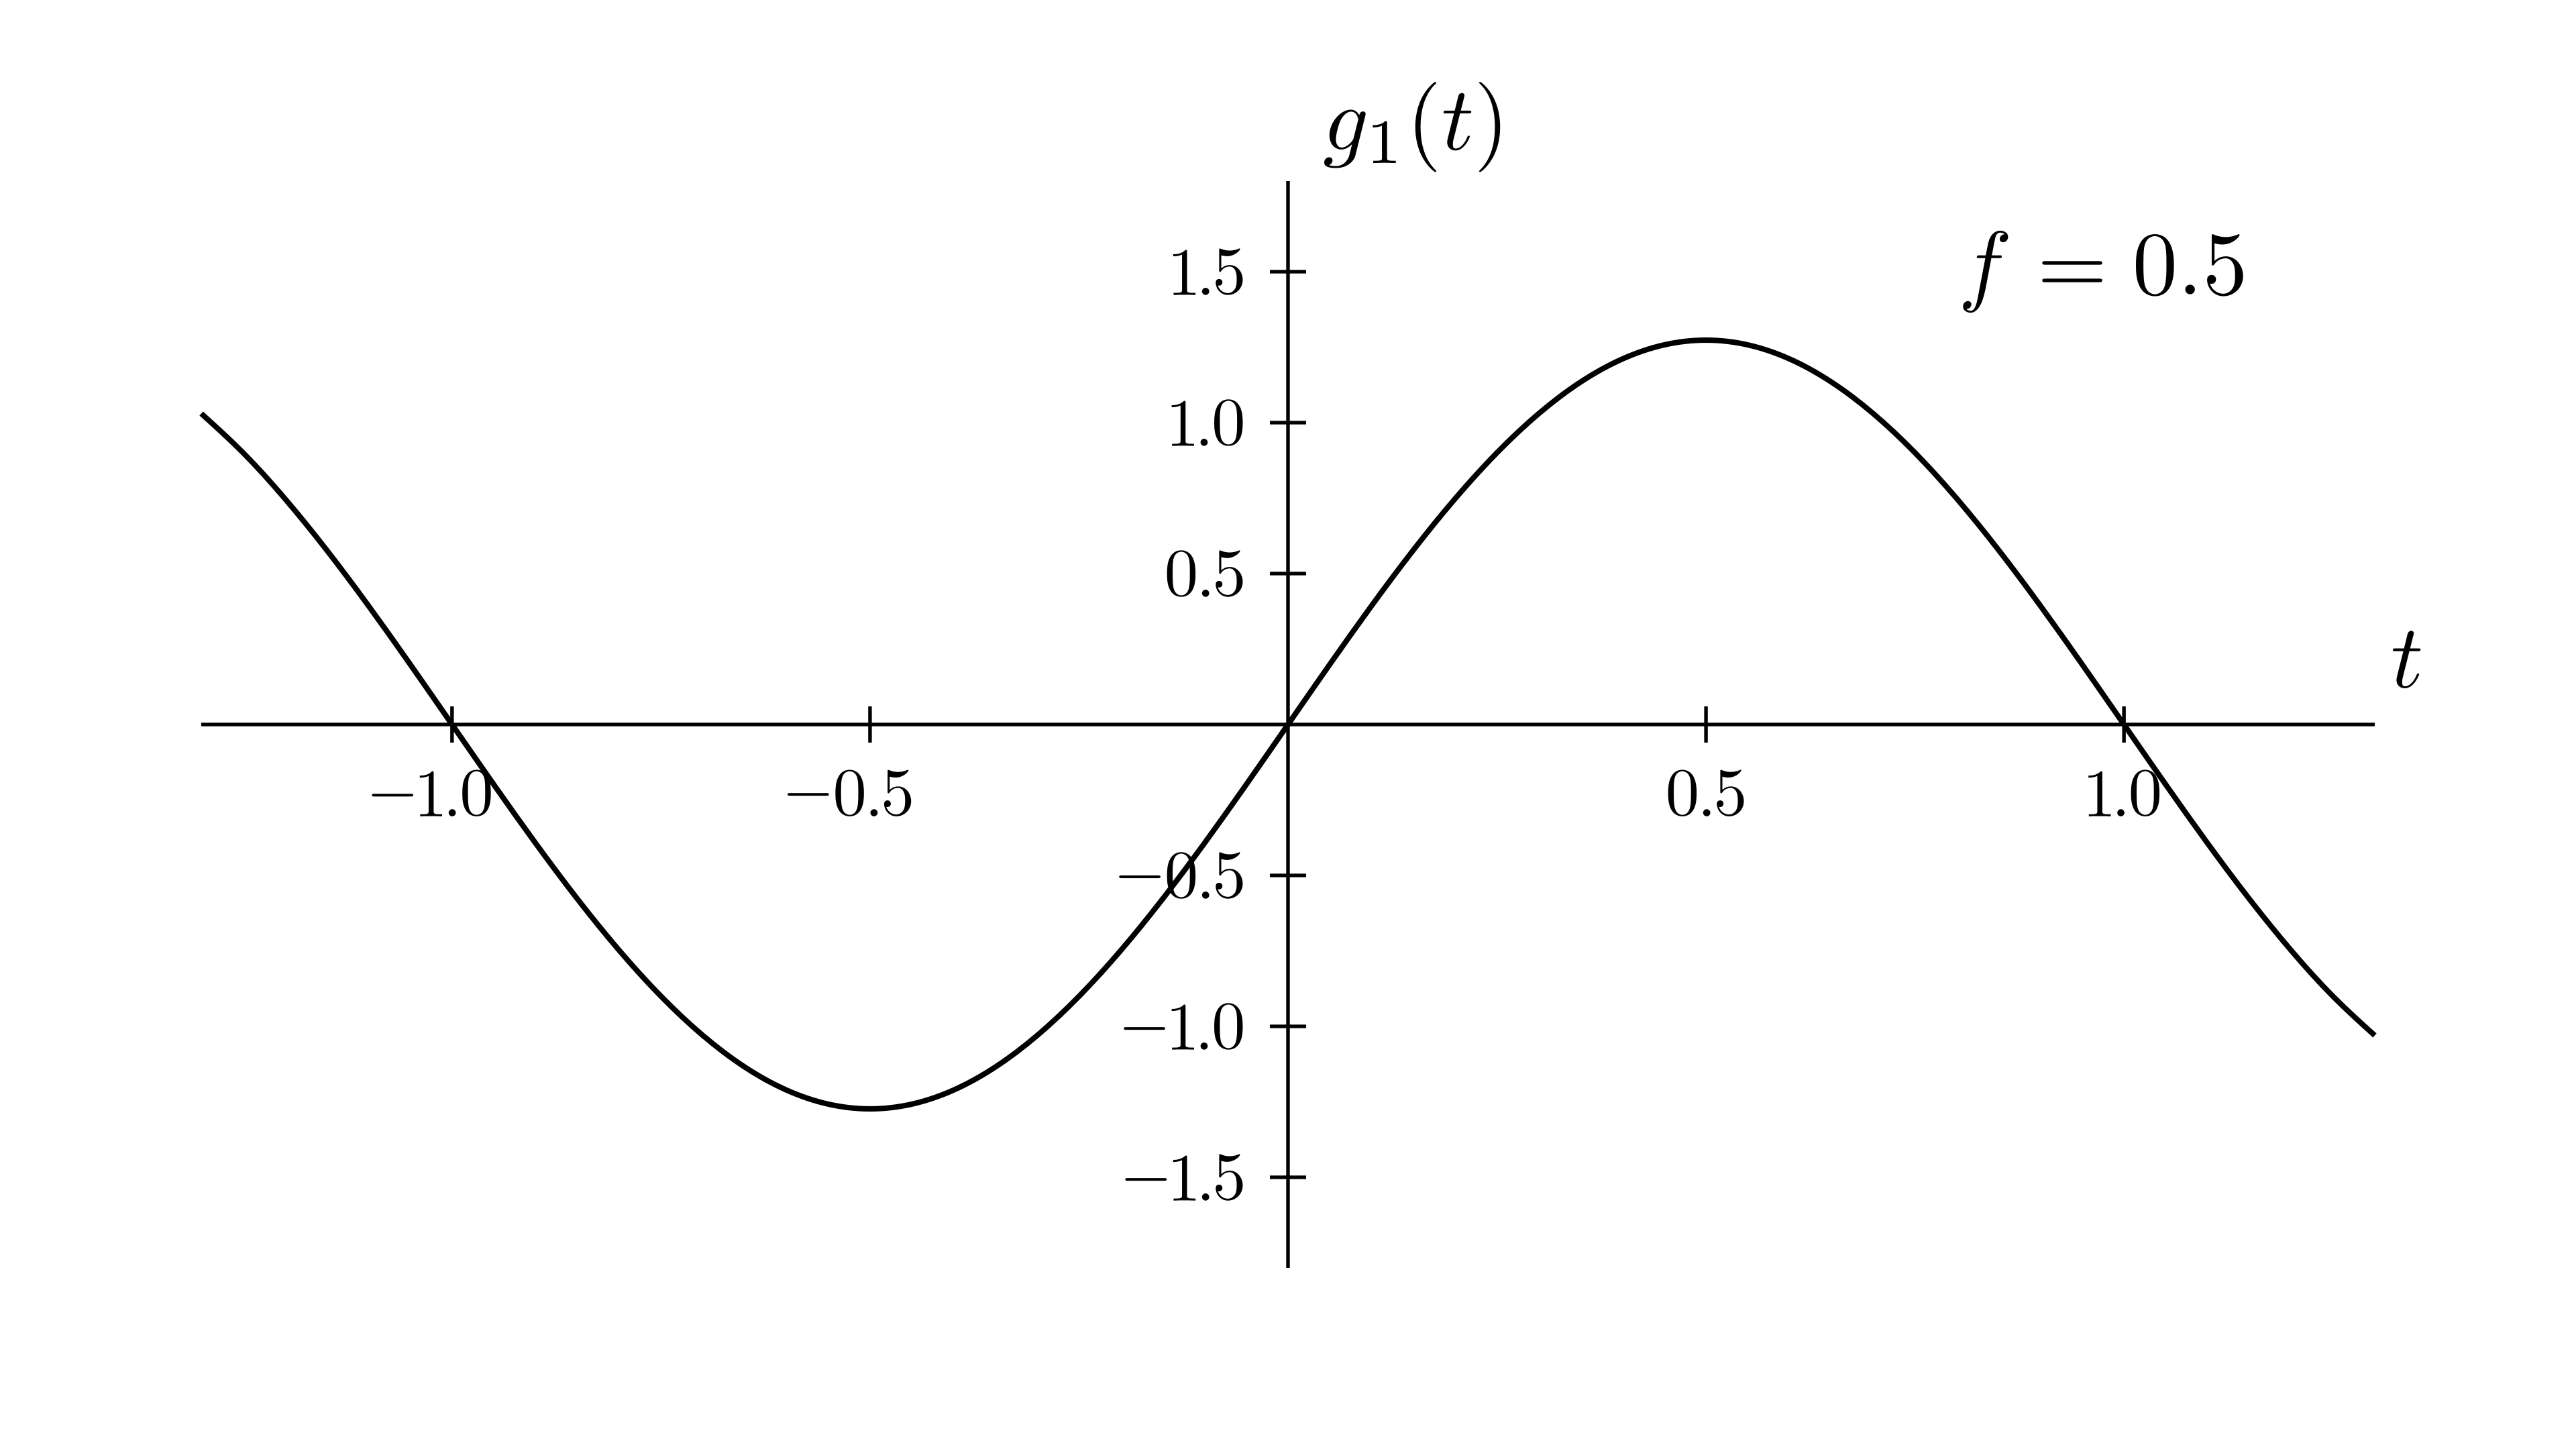
\includegraphics[width=\linewidth,height=0.85\textheight,keepaspectratio]{../assets/first-term-function.png}
	\end{frame}

	% breakdown-7
	\begin{frame}{breaking down a scary looking function}
		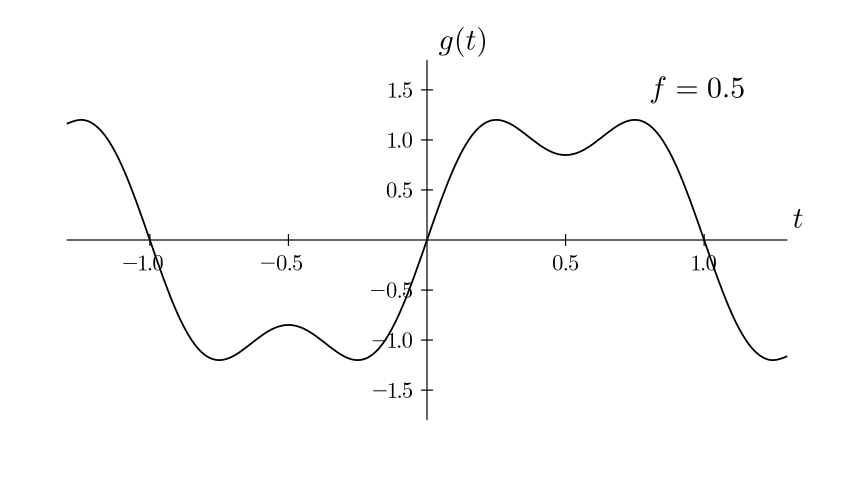
\includegraphics[width=\linewidth,height=0.85\textheight,keepaspectratio]{../assets/second-term-function.png}
	\end{frame}
	
	% breakdown-8
	\begin{frame}{breaking down a scary looking function}
		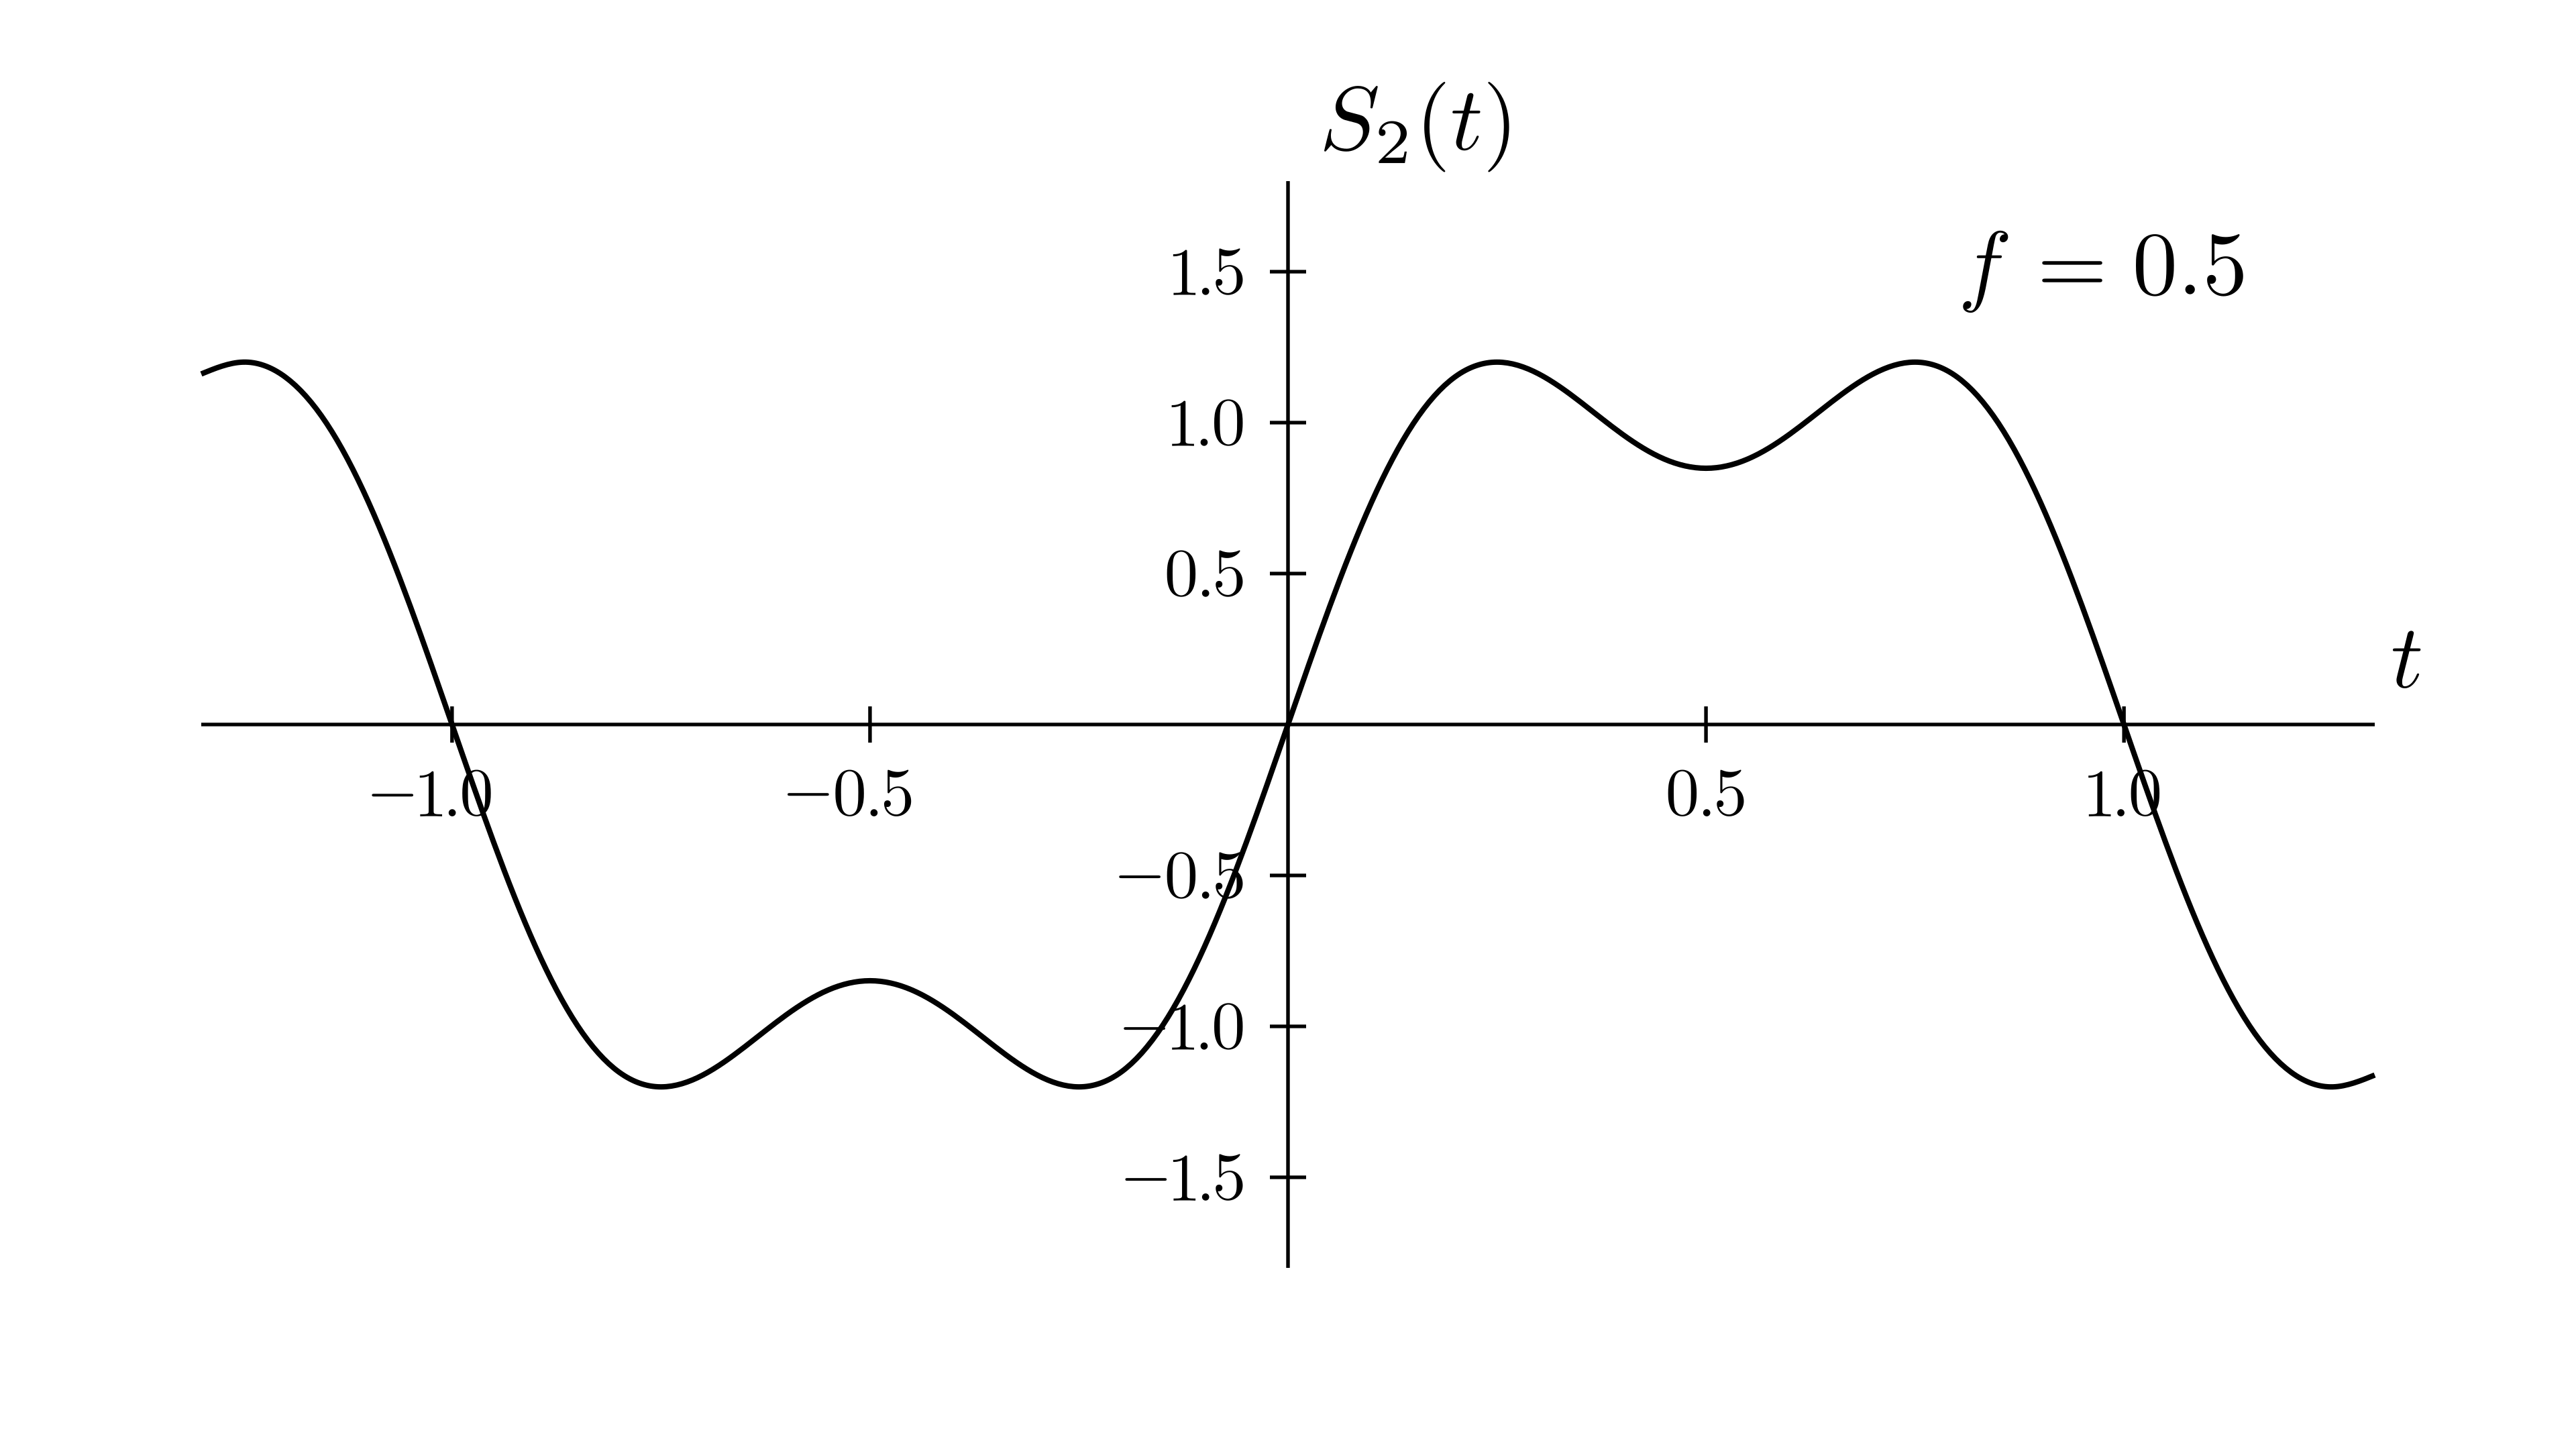
\includegraphics[width=\linewidth,height=0.85\textheight,keepaspectratio]{../assets/sum-two-terms.png}
	\end{frame}
	
	% breakdown-9
	\begin{frame}{breaking down a scary looking function}
		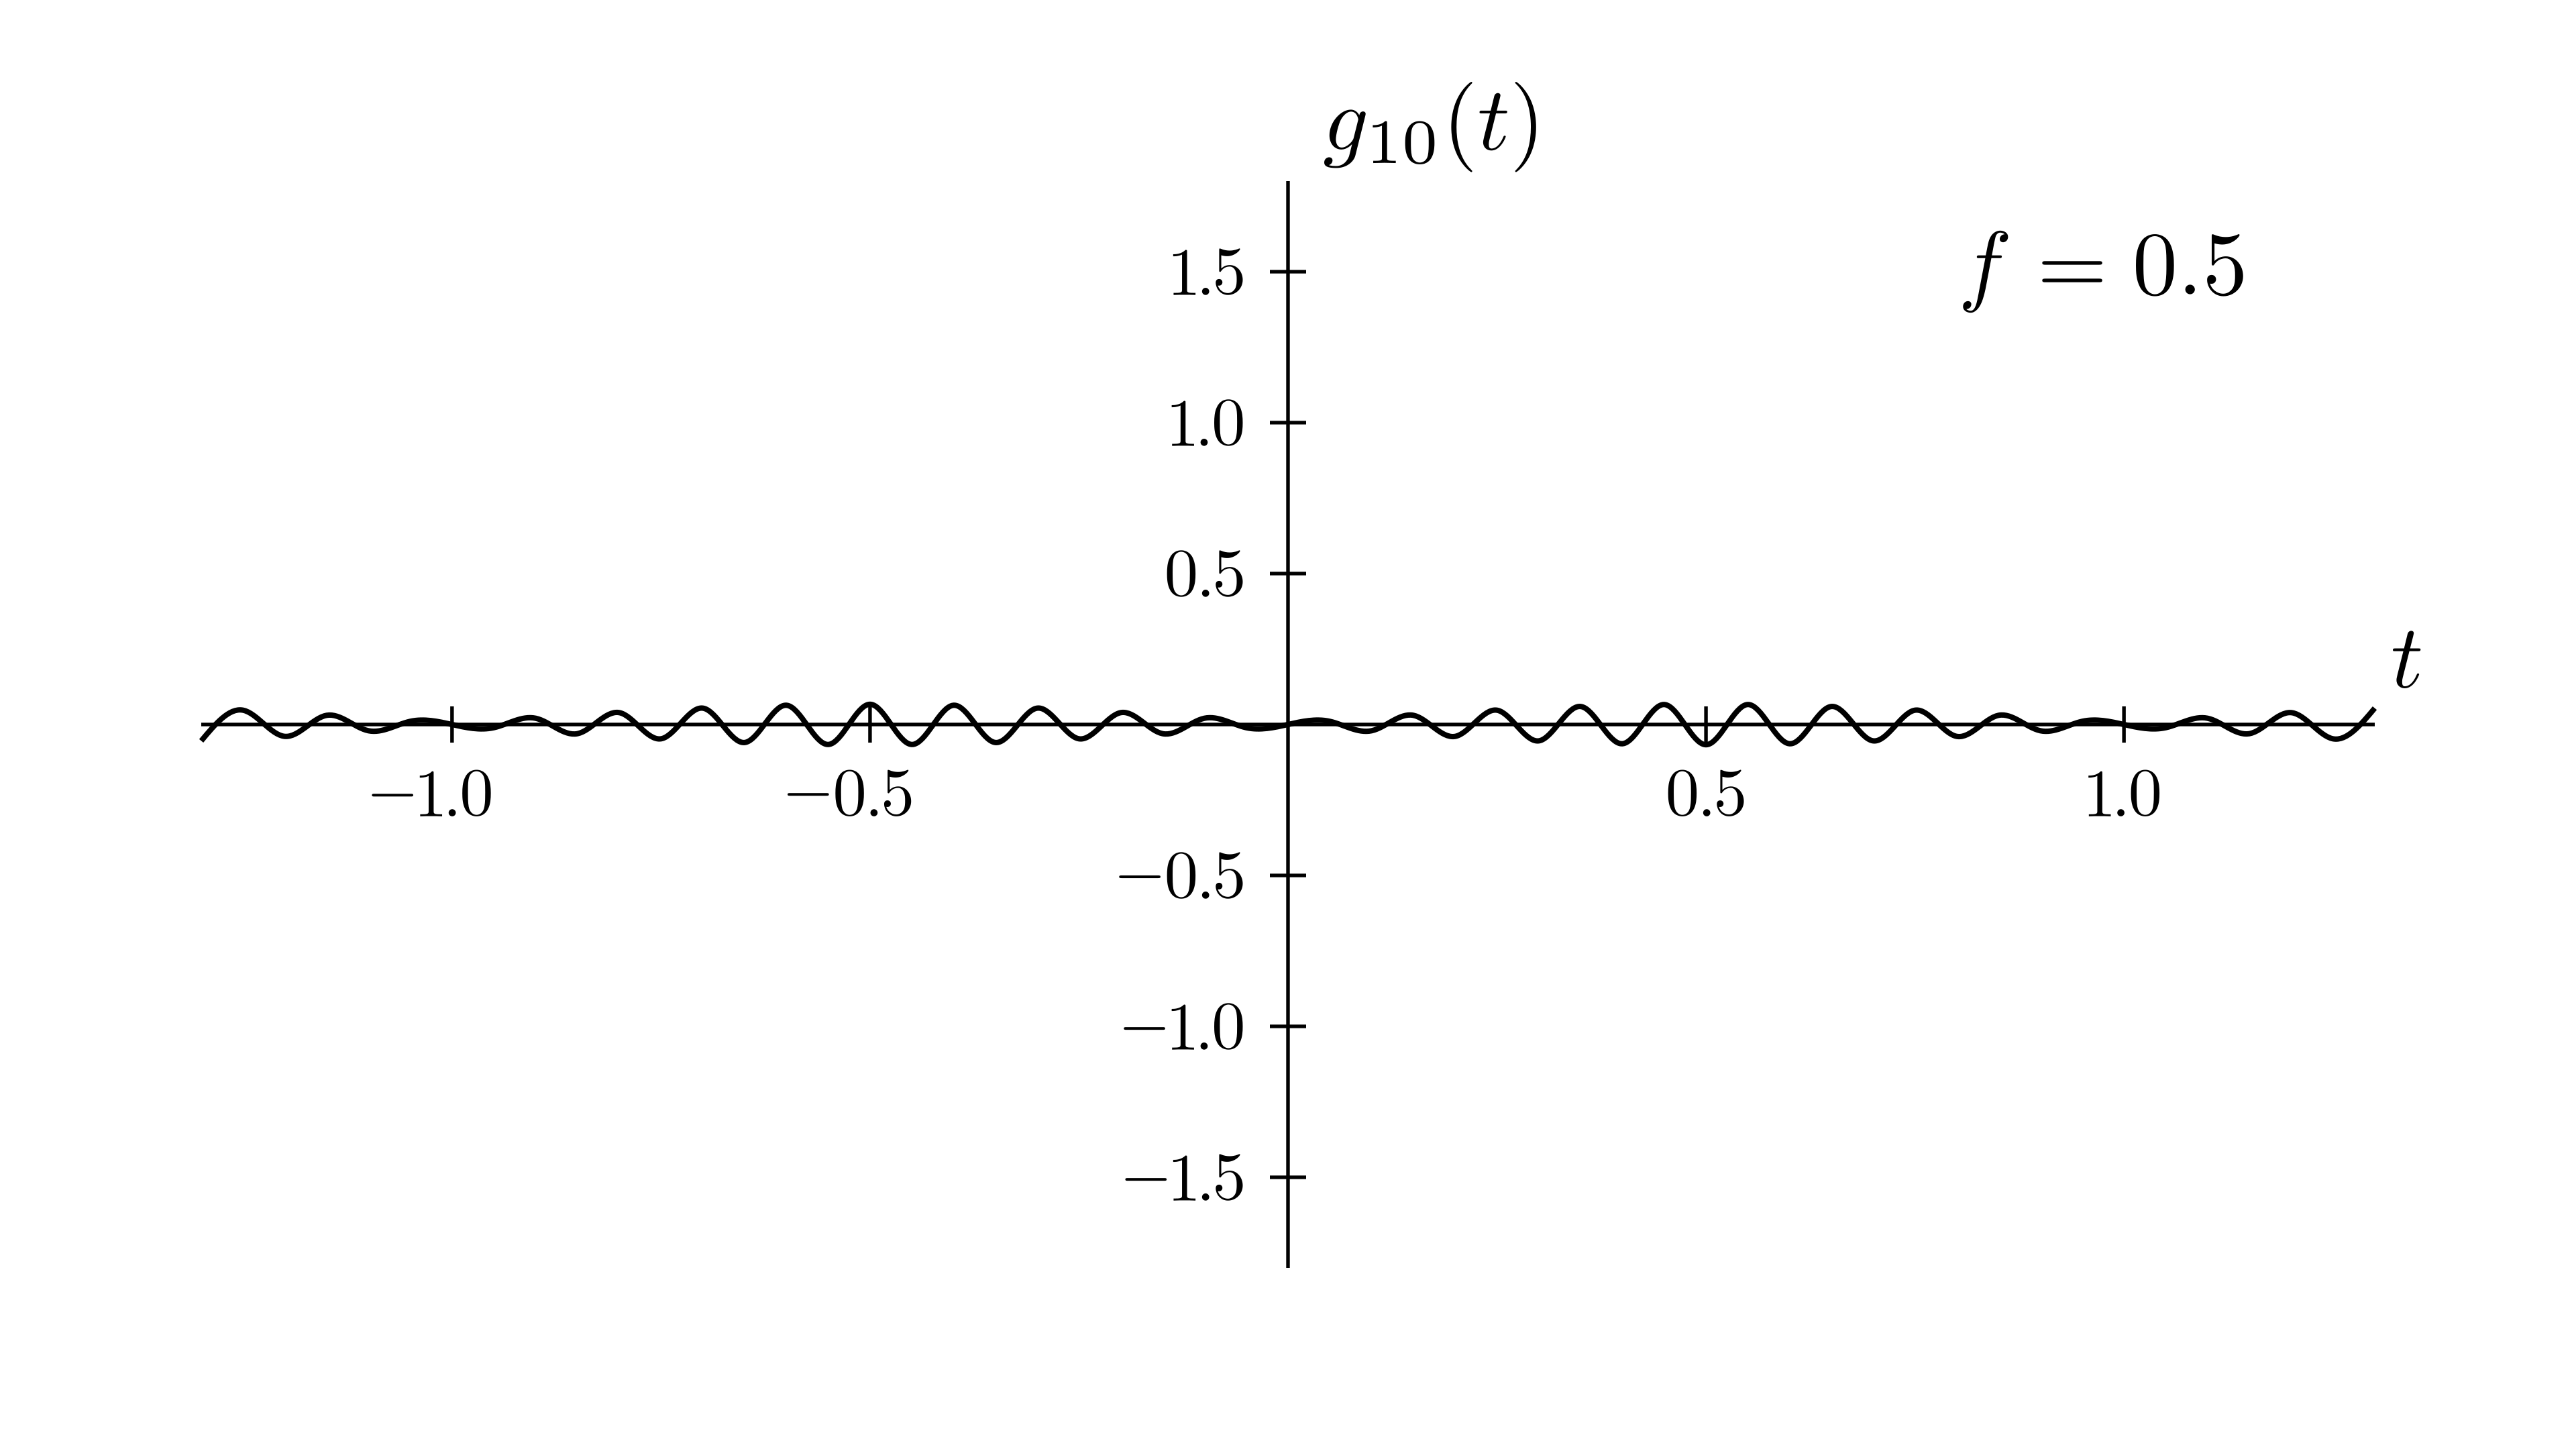
\includegraphics[width=\linewidth,height=0.85\textheight,keepaspectratio]{../assets/tenth-term-function.png}
	\end{frame}
	
	% breakdown-10
	\begin{frame}{breaking down a scary looking function}
		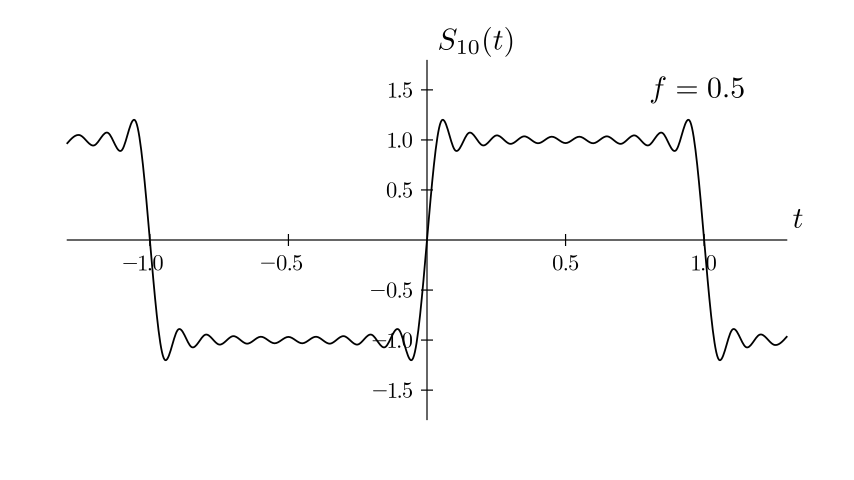
\includegraphics[width=\linewidth,height=0.85\textheight,keepaspectratio]{../assets/sum-ten-terms.png}
	\end{frame}
	
	% arrays-1
	\begin{frame}{vectors (not the math kind), i.e. arrays}
		\begin{itemize}
			\item[] set of pairs $\Rightarrow$ index and value
			\item[] elements (pairs) are conventionally of same memory size
		\end{itemize}
	\end{frame}
	
	% arrays-2
	\begin{frame}{vectors (not the math kind), i.e. arrays}
		\vfill
		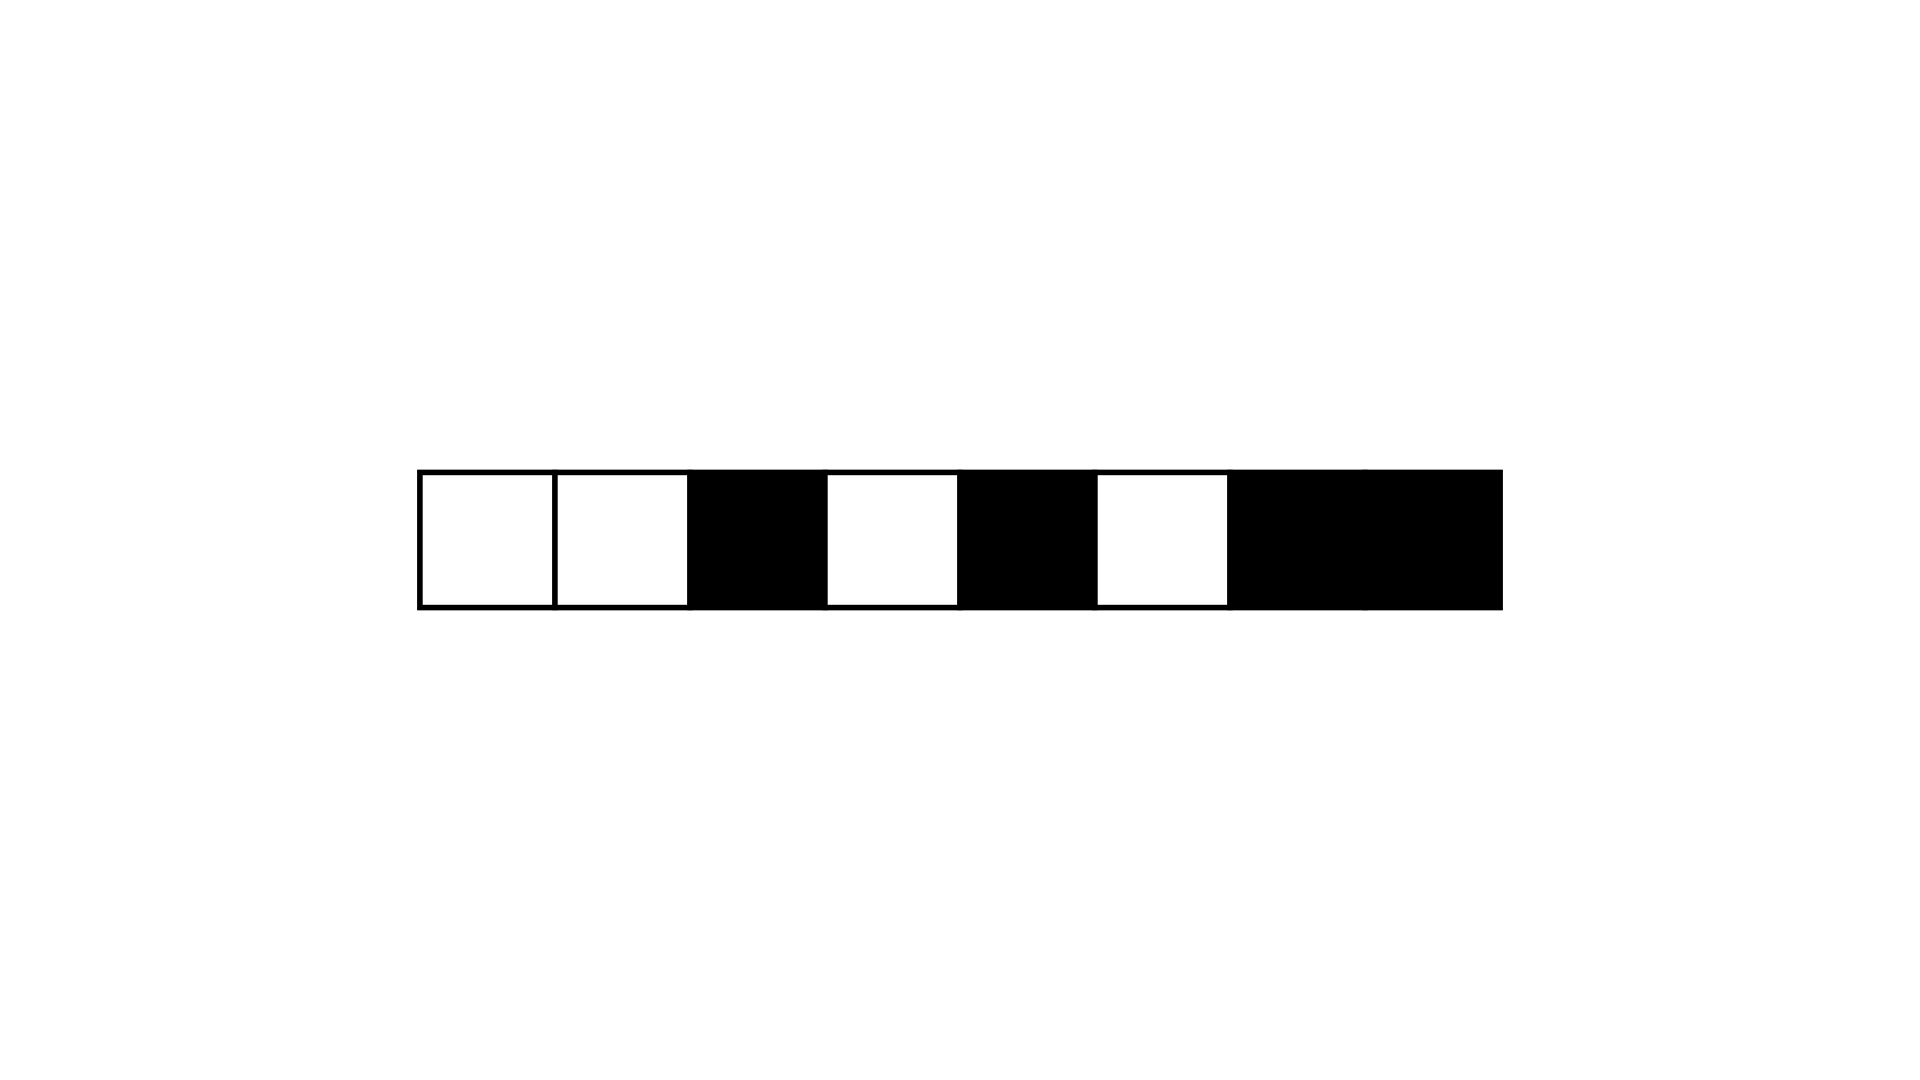
\includegraphics[width=\linewidth,height=0.85\textheight,keepaspectratio]{../assets/1d-array.png}
		\vfill
		\small
			one\_d\_array = [0, 0, 1, 0, 1, 0, 1, 1]
		\vfill
	\end{frame}
	
	% arrays-3
	\begin{frame}{vectors (not the math kind), i.e. arrays}
		\vfill
		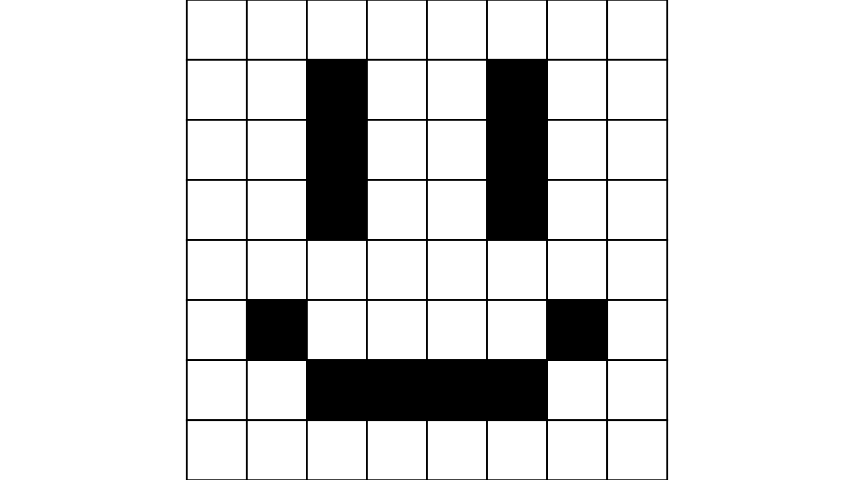
\includegraphics[width=\linewidth,height=0.85\textheight,keepaspectratio]{../assets/2d-array.png}
		\vfill
	\end{frame}
	
	% arrays-4
	\begin{frame}{vectors (not the math kind), i.e. arrays}
		\vfill
		\small
			two\_d\_array = [
			
			[0, 0, 0, 0, 0, 0, 0, 0],
			
			[0, 0, 1, 0, 0, 1, 0, 0],
			
			[0, 0, 1, 0, 0, 1, 0, 0],
			
			[0, 0, 1, 0, 0, 1, 0, 0],
			
			[0, 0, 0, 0, 0, 0, 0, 0],
			
			[0, 1, 0, 0, 0, 0, 1, 0],
			
			[0, 0, 1, 1, 1, 1, 0, 0],
			
			[0, 0, 0, 0, 0, 0, 0, 0]
			
		]
		\vfill
	\end{frame}
	
	% arrays-5
	\begin{frame}{vectors (not the math kind), i.e. arrays}
		\begin{center}
			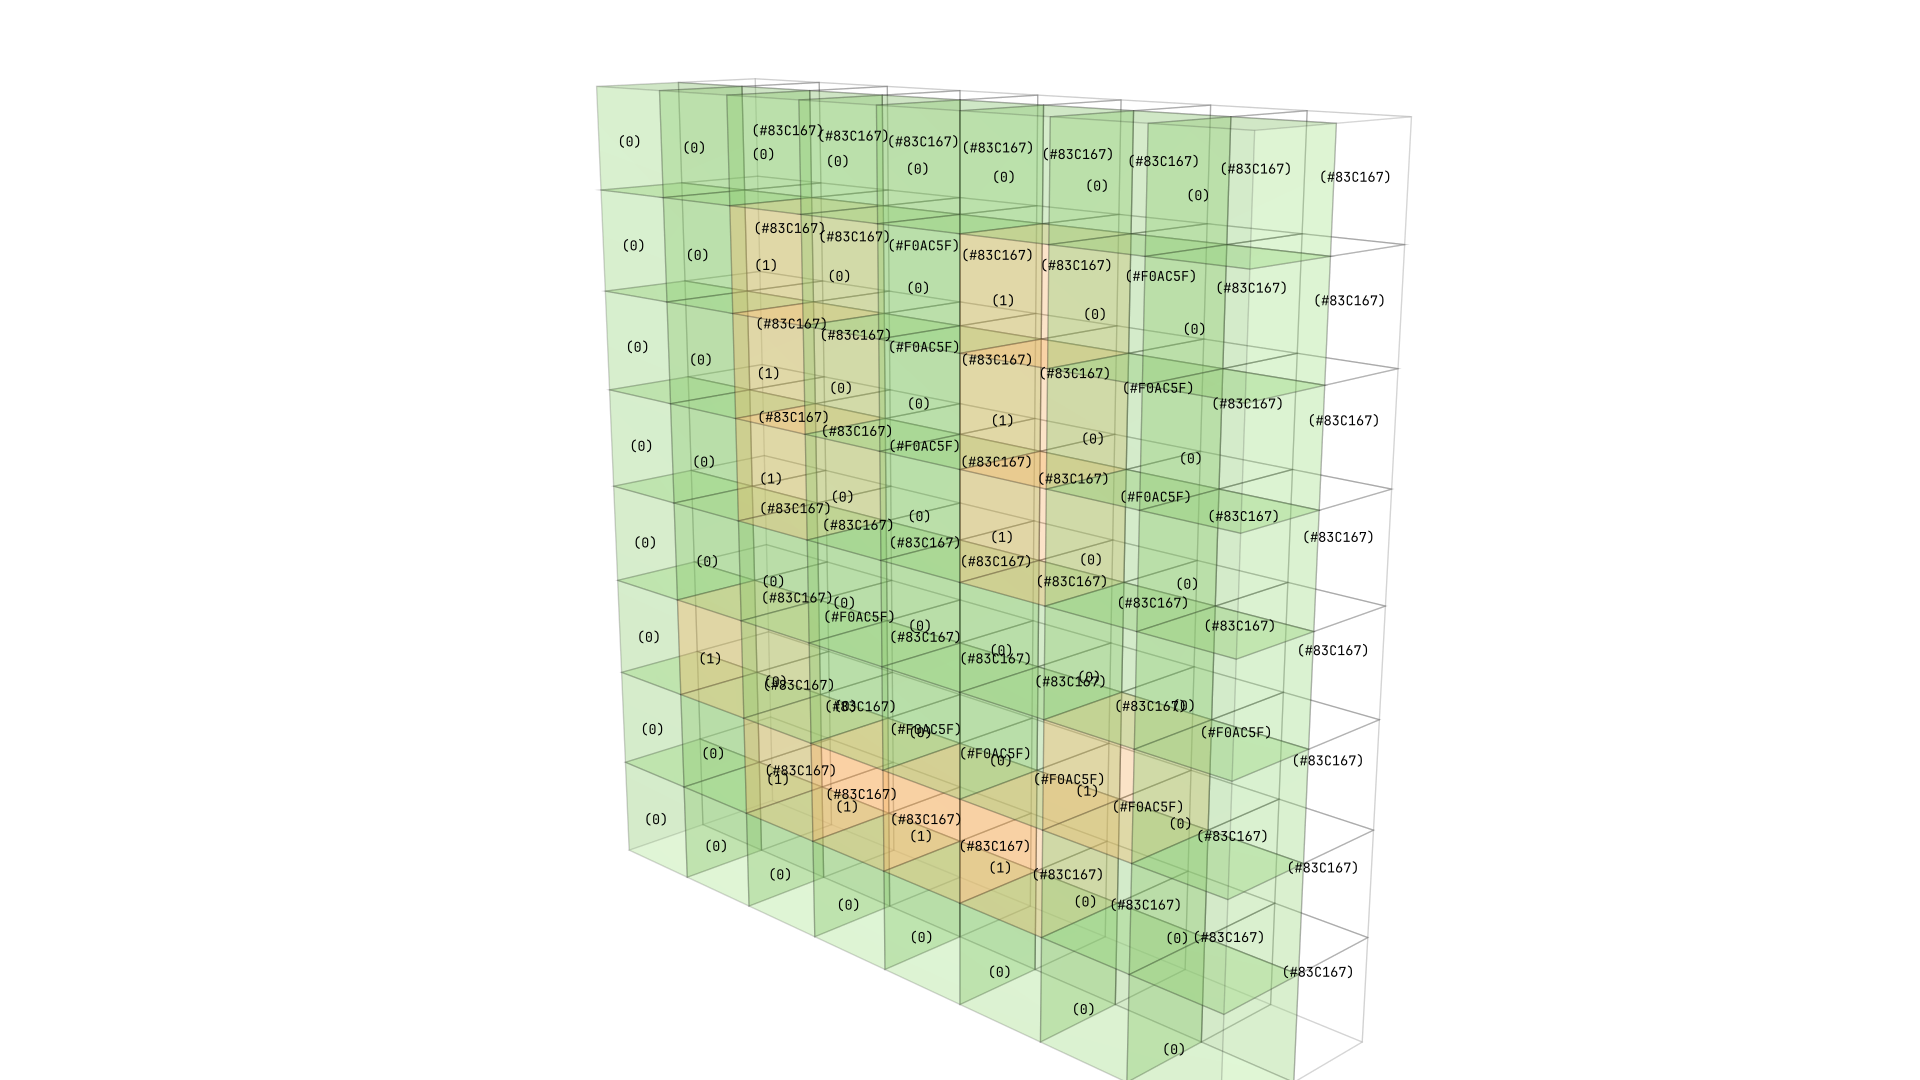
\includegraphics[width=\linewidth,height=0.85\textheight,keepaspectratio]{../assets/3d-array-rotated.png}
		\end{center}
	\end{frame}
	
	% binary-tree-1
	\begin{frame}{binary tree}
		\begin{itemize}
			\item[] data structure expressed as a figurative tree
			\item[] one root node
			\item[] nodes can only have one parent node and at most two children nodes (left and right)
			\item[] foundation for more complex data structures
		\end{itemize}
	\end{frame}
	
	% binary-tree-2
	\begin{frame}{binary tree}
		\begin{center}
			\begin{forest}
				for tree={
					grow=south,
					circle, draw, minimum size=3ex, inner sep=1pt,
					s sep=7mm
				}
				[1
				[7
				[2]
				[6
				[5]
				[11]
				]
				]
				[9
				[9
				[5]
				]
				]
				]
			\end{forest}
		\end{center}
		
		\begin{itemize}
			\item[] an unbalanced and unsorted binary tree
			
			\item[] height = 3 i.e., the number of edges from farthest node to root node (1)
			
			\item[] size = 9, i.e., total number of nodes
		\end{itemize}
	\end{frame}
	
	% traversing-tree-1
	\begin{frame}{binary tree traversal using dfs}
		\begin{itemize}
			\item[] depth first search
			\item[] starts at root, goes down as far as it can, backtracks, explores, etc.
			\item[] to implement we need to create a) the structure and b) the algorithm
		\end{itemize}
	\end{frame}
	
	% traversing-tree-2
	\begin{frame}[fragile]{binary tree traversal using dfs - the structure}
		\begin{lstlisting}[style=pythonstyle]
			class Node:
				def __init__(self, val):
					self.data = val
					self.left = None
					self.right = None
			
			def connect(parent, left=None, right=None):
				parent.left = left
				parent.right = right
		\end{lstlisting}
	\end{frame}
	
	% traversing-tree-3
	\begin{frame}[fragile]{binary tree traversal using dfs - the structure}
		\begin{lstlisting}[style=pythonstyle]
			firstNode = Node(1)
			secondNode = Node(7)
			thirdNode = Node(9)
			
			connect(firstNode, secondNode, thirdNode)
		\end{lstlisting}
	\end{frame}
	
	% traversing-tree-4
	\begin{frame}[fragile]{binary tree traversal using dfs - the algorithm}
		\begin{lstlisting}[style=pythonstyle]
			def depth_first_search(root, value):
				if root is None:
					return False
				root.visited = True
			
				if root.data == value:
					return True
			
				l_res = depth_first_search(root.left, value)
				r_res = depth_first_search(root.right, value)
			
				return l_res or r_res
		\end{lstlisting}
	\end{frame}
	
	% matrices-1
	\begin{frame}{matrices}
		\begin{itemize}
			\item[] math implementation of arrays, in a way
			\item[] 2d/3d transformations in graphics (scaling, rotation, translation) 
			\item[] $P=(1,2)$ can also be expressed as $P=\begin{bmatrix} 1 \\ 2 \end{bmatrix}$
			\item[] $M = \begin{bmatrix} 3 & 2 \\ 4 & 1 \end{bmatrix}$
			\item[] $P_m=M\cdot P = \begin{bmatrix} 3 & 2 \\ 4 & 1 \end{bmatrix}\cdot \begin{bmatrix} 1 \\ 2 \end{bmatrix} = \begin{bmatrix} 3 \cdot 1 + 4 \cdot 1 \\ 2 \cdot 2 + 1 \cdot 2 \end{bmatrix}$
		    \item[] $P_m=(7,6)$
		\end{itemize}
	\end{frame}
	
	% big-o-1
	\begin{frame}{big o}
		\begin{itemize}
			\item[] o stands for ordnung, order of approximation
			\item[] how different algorithms scale and grow in terms of complexity
			\item[] time / input $\Rightarrow$ output
			\item[] ignores terms but the one that "grows" the quickest
		\end{itemize}
	\end{frame}
	
	% big-o-2
	\begin{frame}{big o}
		constant $O(1)$
		\begin{itemize}
			\item[] same amount of time, no matter the size of hte input
			\item[] looking up value at index
		\end{itemize}
		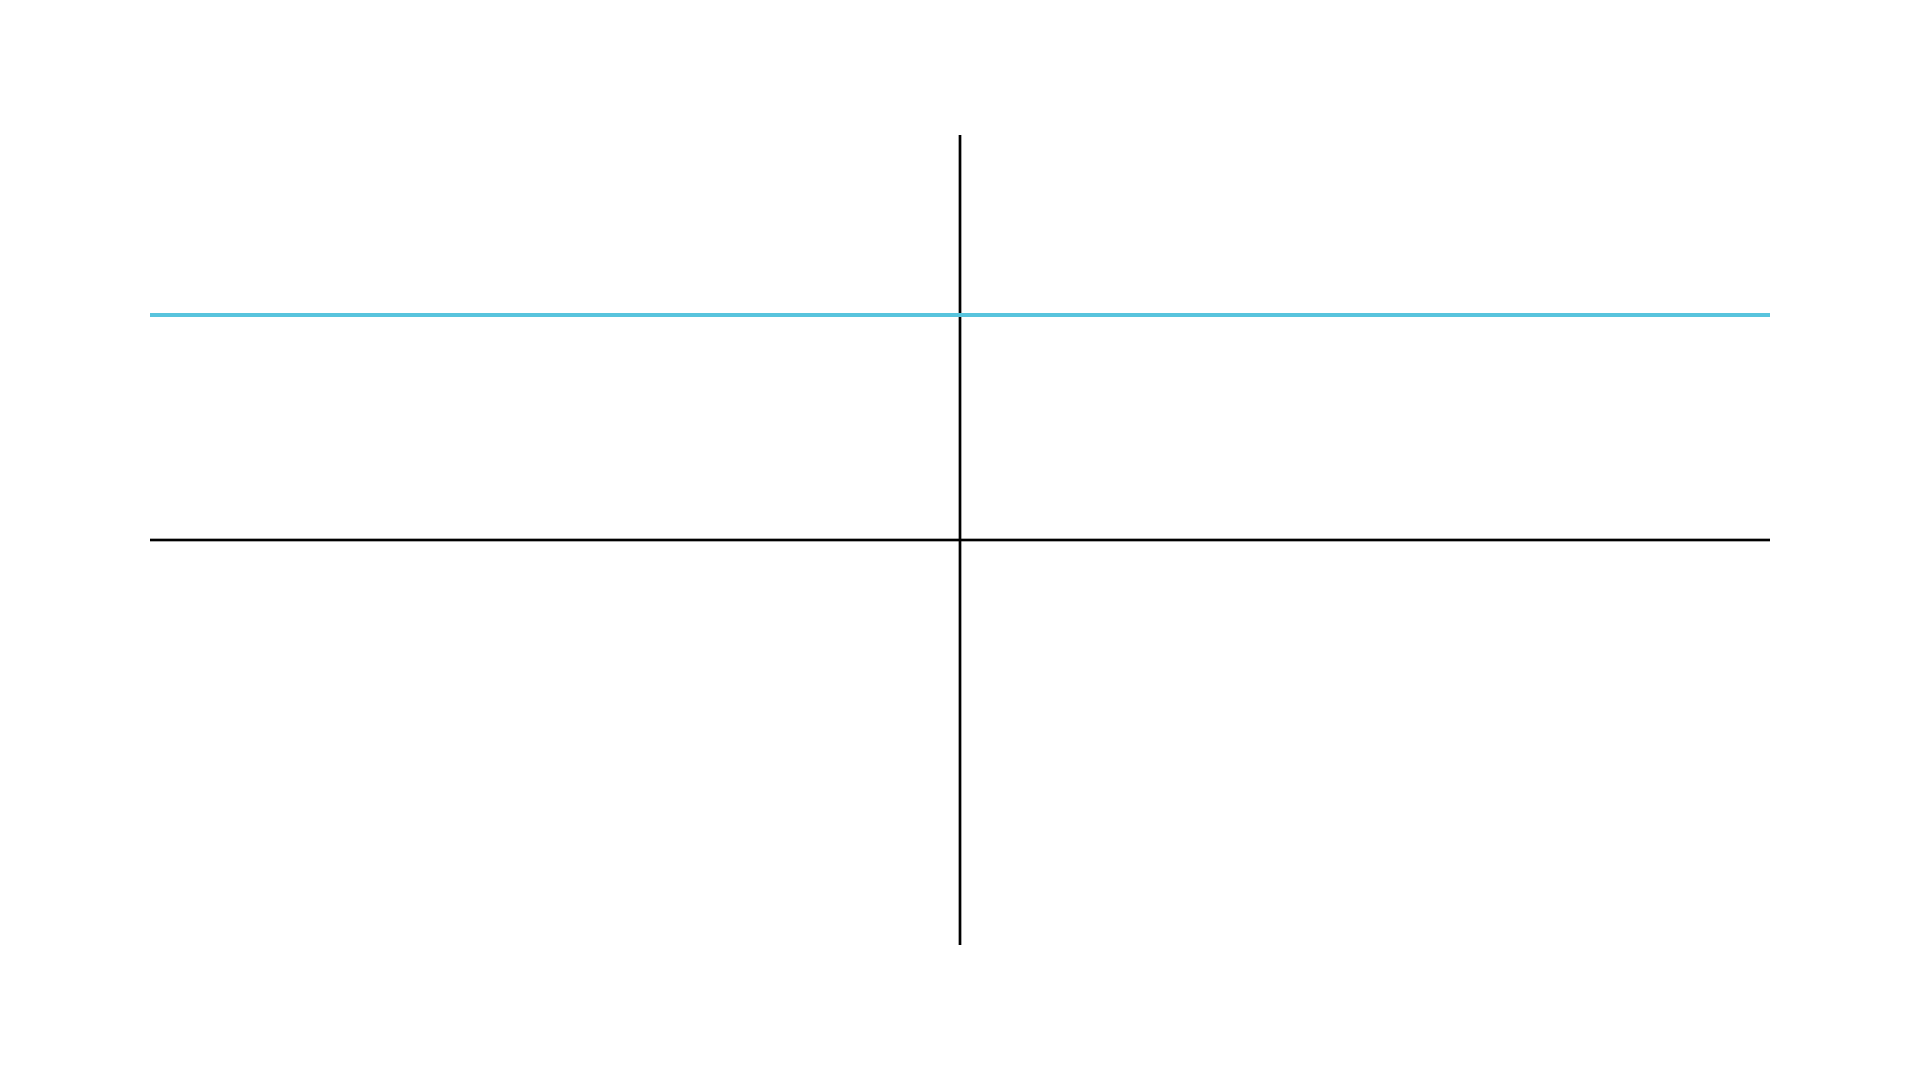
\includegraphics[width=\linewidth,height=0.85\textheight,keepaspectratio]{../assets/constant-scale.png}	
	\end{frame}
	
	% big-o-3
	\begin{frame}{big o}
		linear $O(n)$
		\begin{itemize}
			\item[] grows linearly with the size of the input
			\item[] traversing a binary tree ;)
		\end{itemize}
		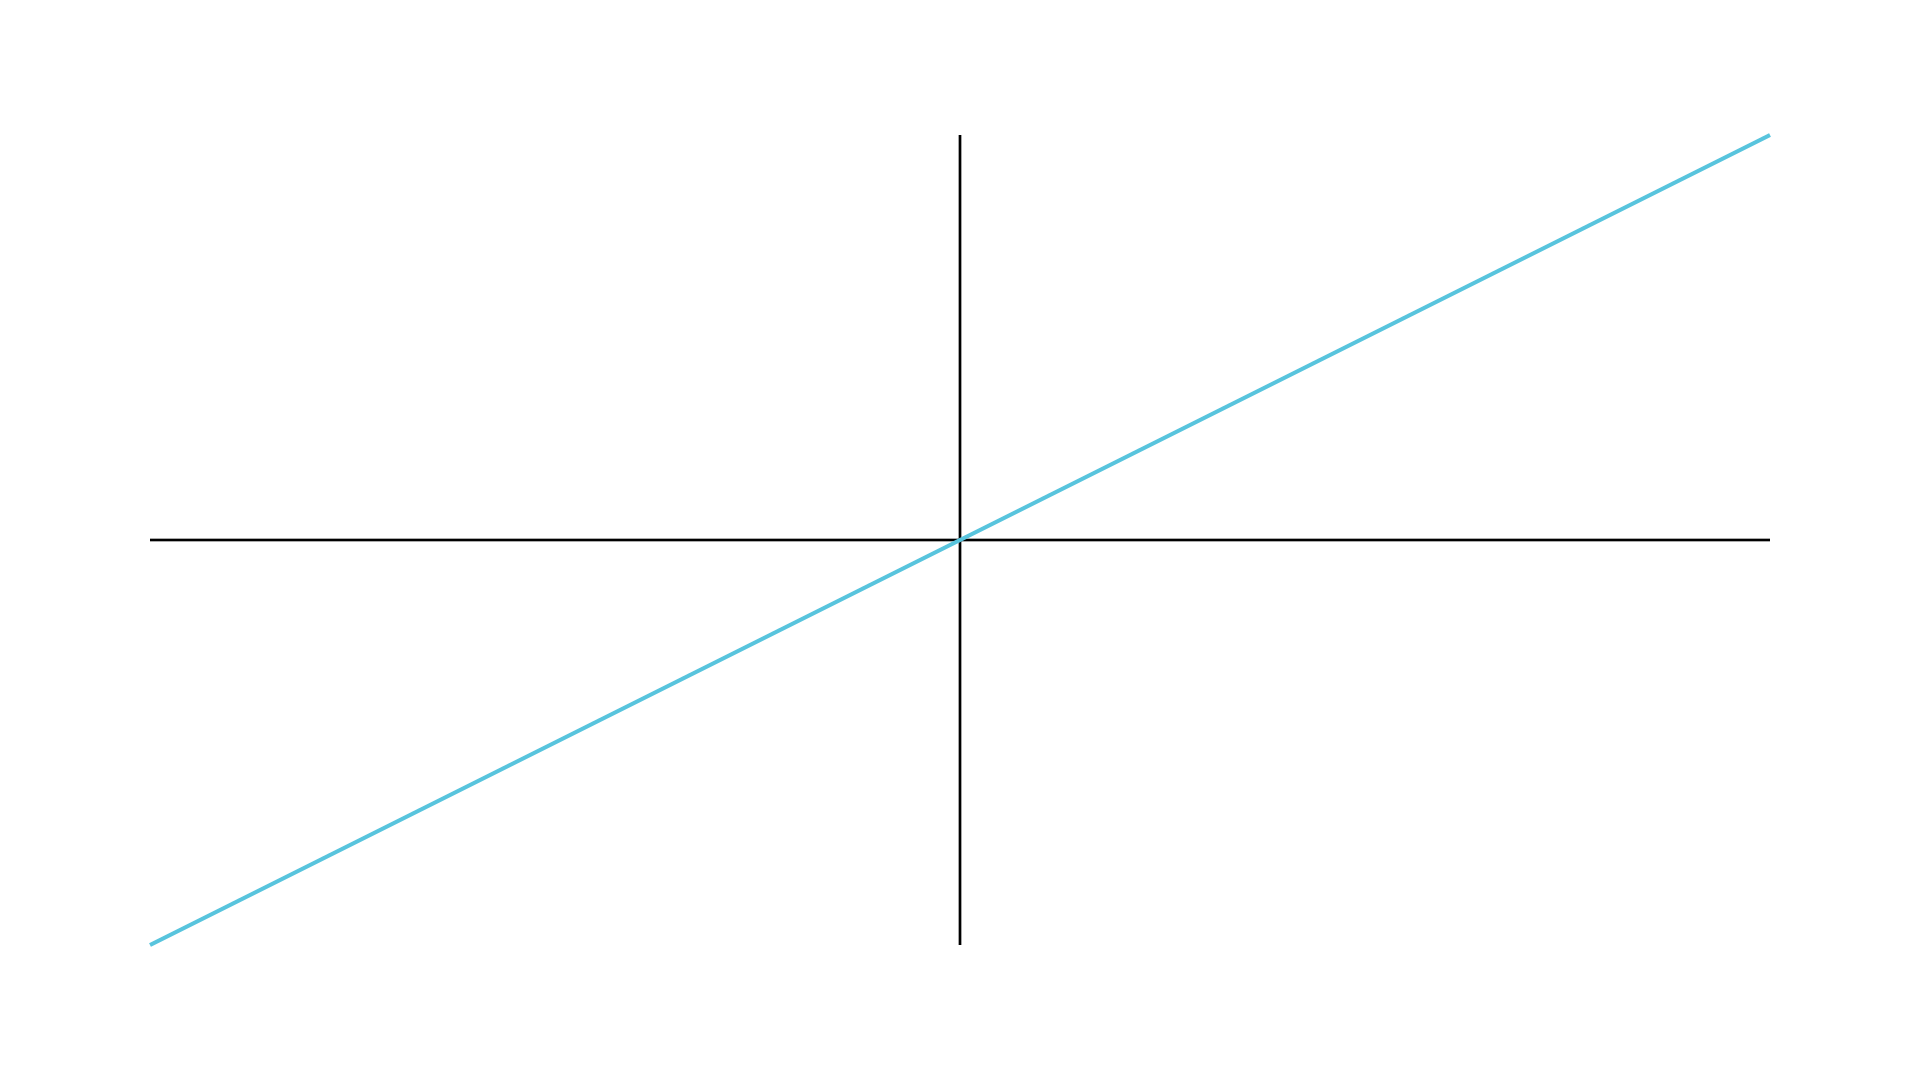
\includegraphics[width=\linewidth,height=0.85\textheight,keepaspectratio]{../assets/linear-scale.png}	
	\end{frame}
	
	% big-o-4
	\begin{frame}{big o}
		logarithmic $O(\log n)$
		\begin{itemize}
			\item[] proportional to the logarithm of the input size
			\item[] binary search algorithm
		\end{itemize}
		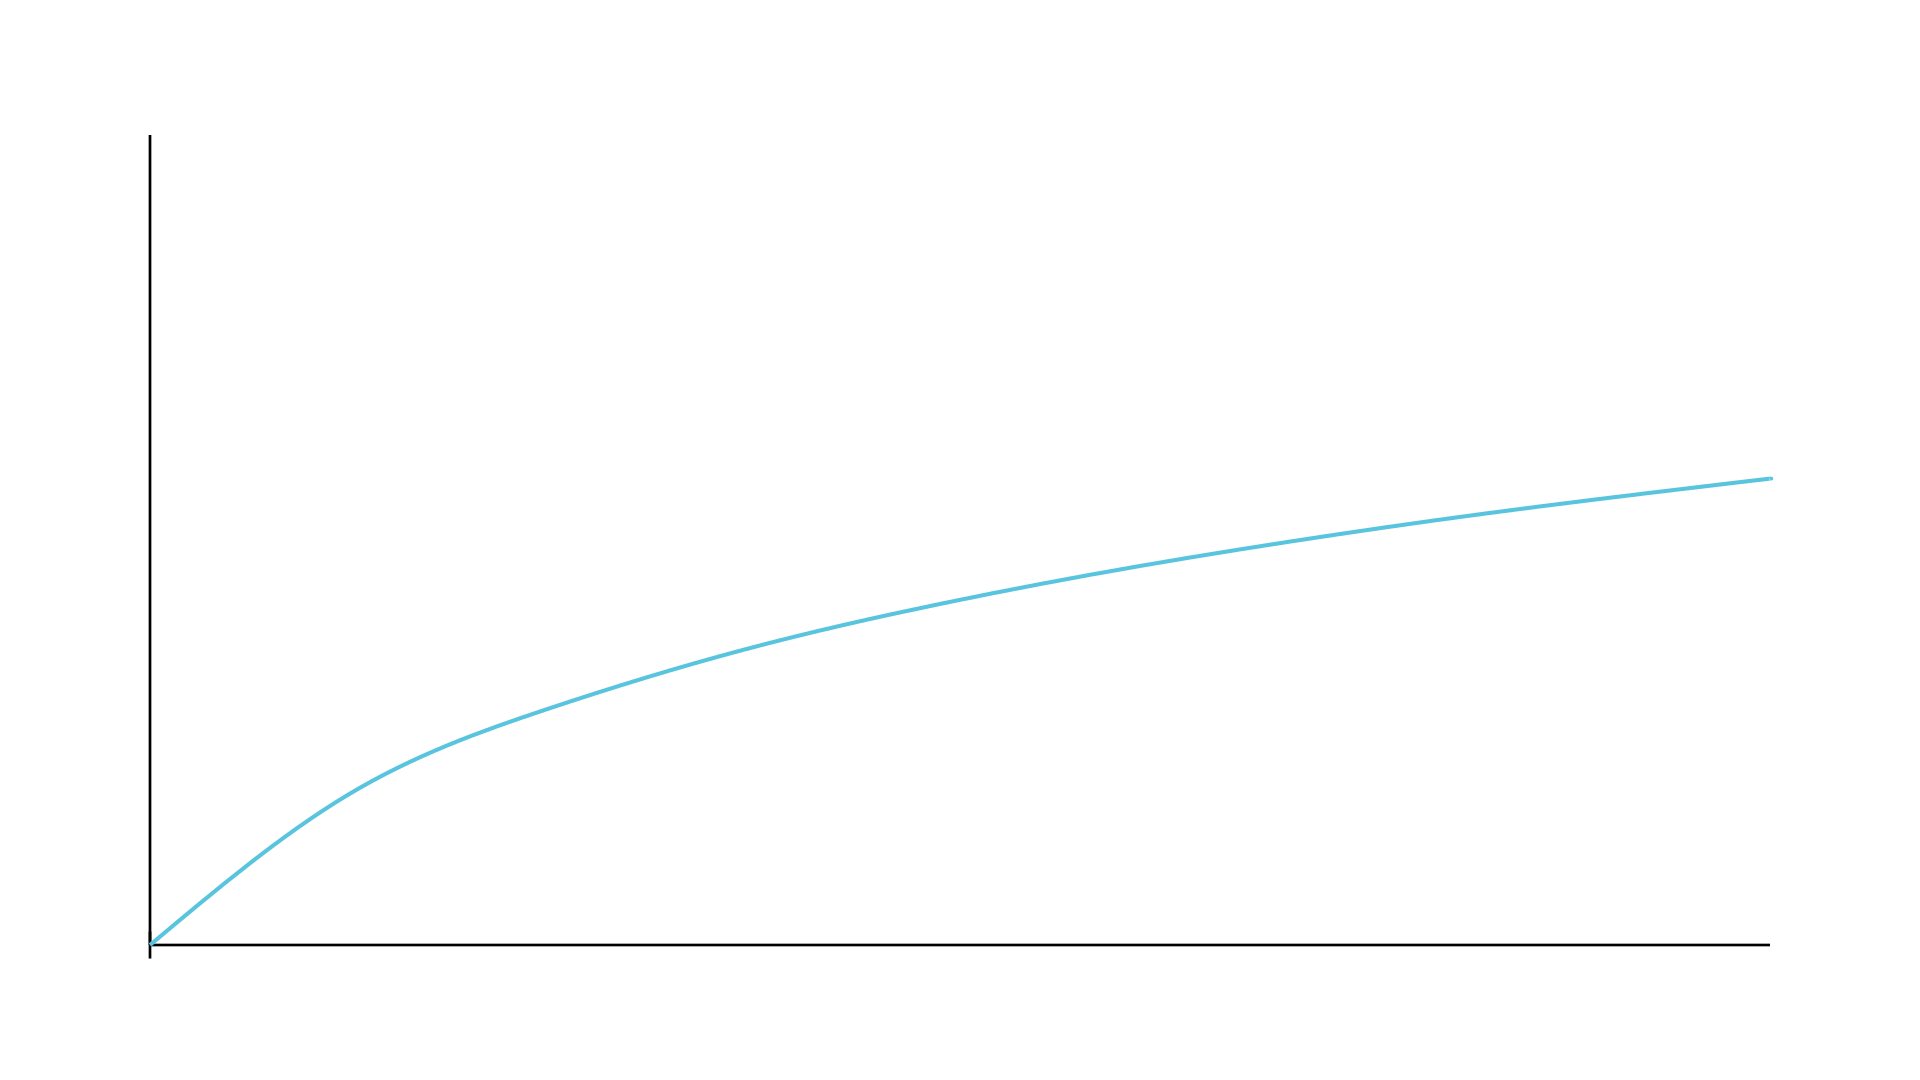
\includegraphics[width=\linewidth,height=0.85\textheight,keepaspectratio]{../assets/log-scale.png}	
	\end{frame}
	
	% big-o-5
	\begin{frame}{big o}
		quadratic $O(n^2)$
		\begin{itemize}
			\item[] proportional to the square of the input
			\item[] for example bubble sort
		\end{itemize}
		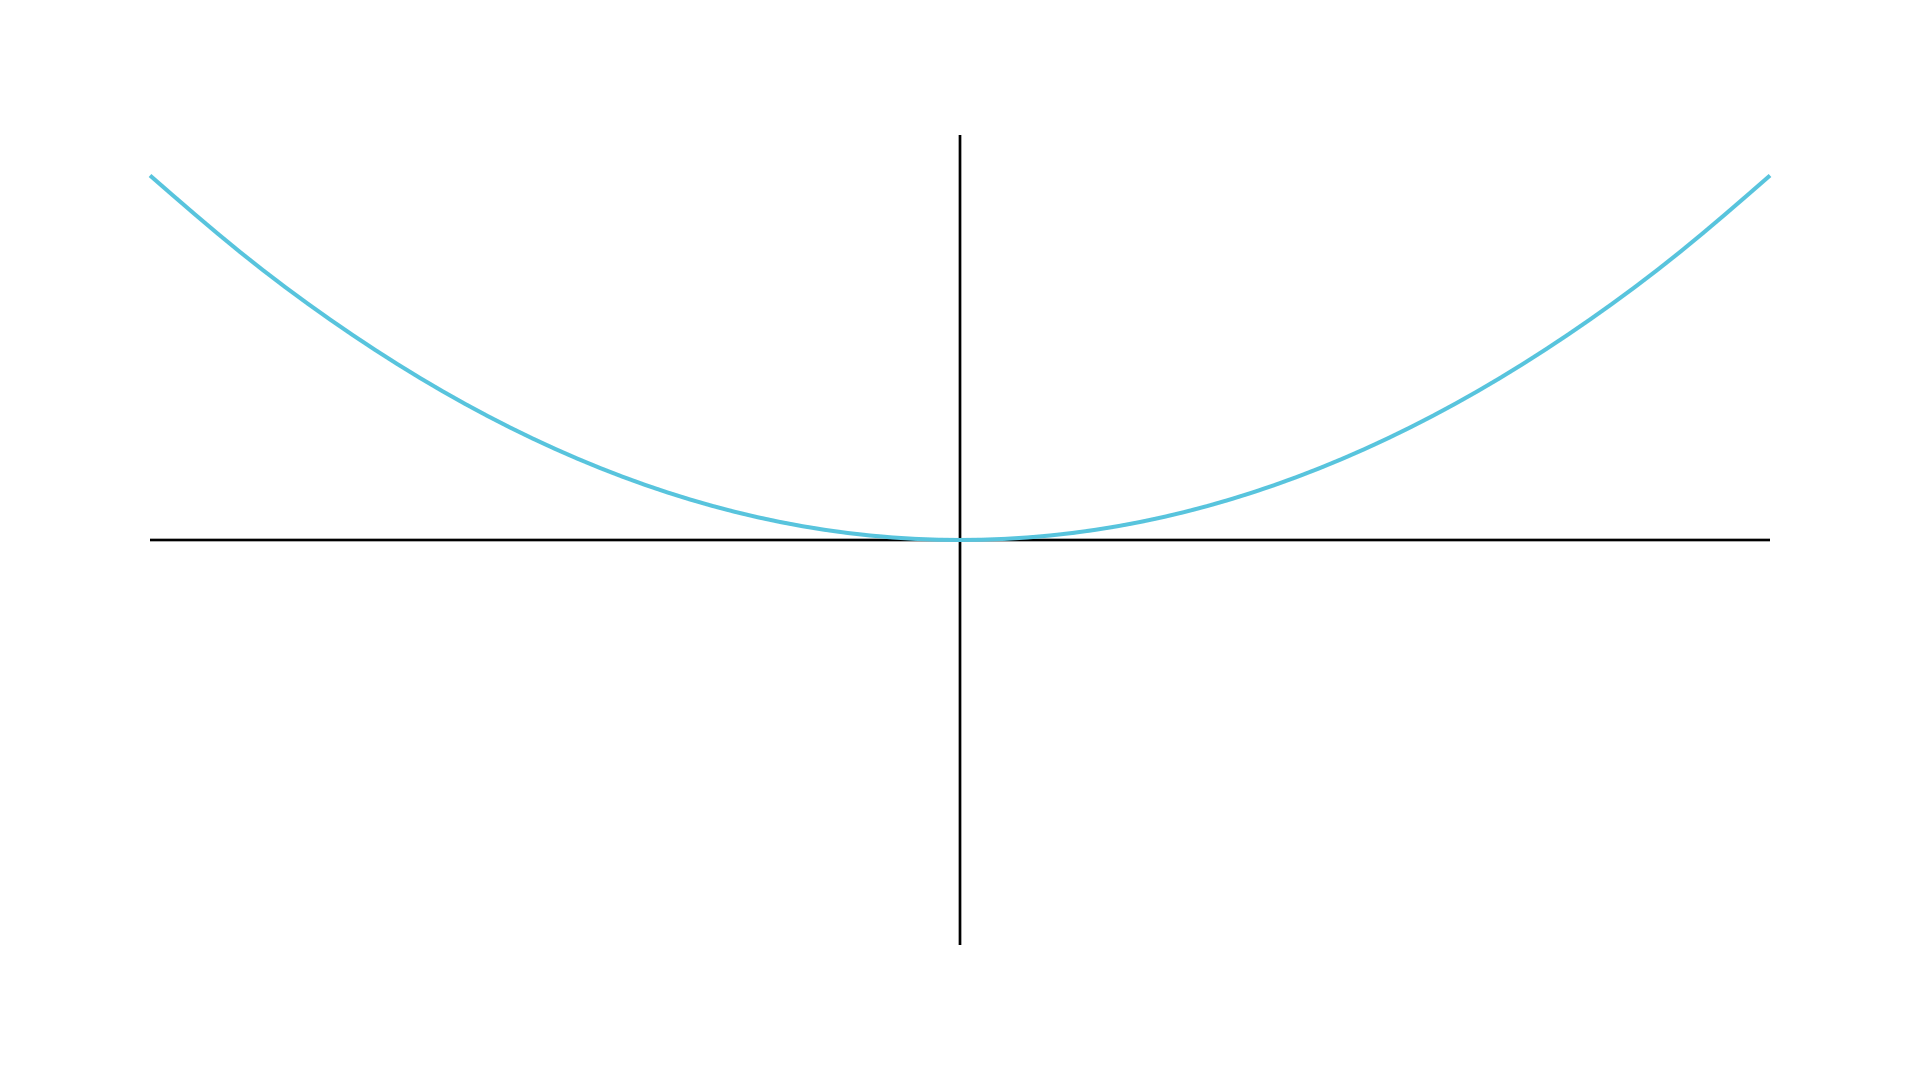
\includegraphics[width=\linewidth,height=0.85\textheight,keepaspectratio]{../assets/quadratic-scale.png}	
	\end{frame}
\end{document}
